\section{HLS based BFS optimization} \label{sec:bfs-opt}
This work centers the HLS based BFS optimization on FPGAs. 
In order to guide the HLS tools to generate efficient hardware, 
we propose a series of methods to regularize the irregular memory 
accesses and dynamic data paths in BFS algorithm. 

\subsection{Irregularity in BFS Structure}
The basic pipelined BFS structure with classical top-down traverse 
is presented in Figure \ref{fig:base-bfs}. It can be roughly 
divided into four pipeline stages. In the first stage, it reads 
frontier from memory. Then it passes the frontier to the second stage
via the OpenCL channel for further inspection. In the second stage, 
frontier neighbors will be inspected from the graph data. While the 
graph is stored as compressed sparse row (CSR) format which has a row 
pointer array (RPA) containing the edge index starting position of each 
vertex and a column index array (CIA) which is essentially the incoming/outgoing 
neighboring vertex indices, the second stage must go through the RPA read and 
CIA read sequentially. When the frontier neighbors are 
drained from memory, the second stage then forwards them to the third stage.
In the third stage, the each neighboring vertex will be checked if it is 
already visited in previous BFS iterations. If the vertex is unvisited, 
it will be considered as frontier in next BFS iteration. The corresponding 
vertex status will be set and the vertex index will be sent to the last stage.
In the last stage, the vertex indices will be written to memory one 
after another.

\begin{figure}
\center{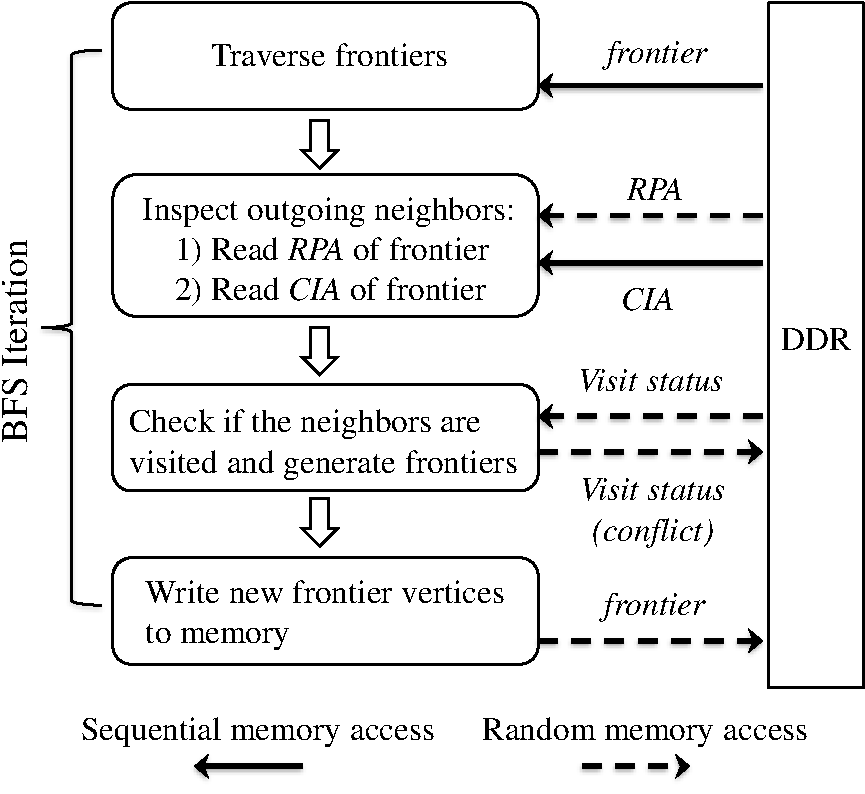
\includegraphics[width=0.75\linewidth]{base-bfs}}
    \caption{Baseline pipelined BFS}
\label{fig:base-bfs}
\end{figure}

The basic BFS structure is well pipelined, but we notice that it involves many 
random memory accesses. In the second stage, as the vertex indices in the frontier 
are usually not continuous, thus the RPA read becomes random. For vertices with 
larger degree, the CIA read can be considered as sequential memory access. Nevertheless, 
the vertex degree can be a random integer, so the CIA read is aligned to 
the vertex index data width (4 bytes in this work) and the bandwidth utilization of 
the sequential memory access remains limited. In the third stage, when the status array 
is located in the memory, the status read is also random. When the vertex is un-visited, 
random write is also required. In the last stage, frontier vertices write is performed one 
after another, it is also random memory access by default. These random memory access 
essentially leads to low meory bandwidth utilization. 

While the data paths in the first, second and fourth pipeline stages are parallel,
the third pipeline stage can not be easily parallelized. Basically, the neihgbors of 
the different frontier vertices may be overlapped. When the frontier vertices are 
processed in parallel, they may update the same vertex status and result in write 
conflict. Worse still, more parallel random accesses will not improve the memory 
bandwidth utilization and increase the average memory access latency instead. 
This stage soon becomes the performance bottleneck. Keeping the vertex status on-chip 
may alleviate the memory access bottleneck, but it is difficult to synchronize the 
vertex status in parallel using HLS. This also prevents the parallelization in the 
other pipeline stages. The authors xx proposed to build a crossbar based shuffling 
between the second stage and the thrid stage. However, the complex logic increases the 
initiation interval (II) dramatically and the overall accelerator performance degrades.

In order to address this problem, we proposed the following optimization methods 
to regularize the memory accesses as well as the data paths so that it can be 
efficiently implemented by the HLS tools. 1) We reorder the edges of the graphs and insert 
padding data with pre processing. It essentially batches the edges and ensures 
no write conflict in each batch. 2) We use bitmap to store the vertex visiting status and 
keep the bitmap in on-chip memory. Meanwhile the bitmap is divided into parallel banks 
based on the pre processing and parallel data paths can operate on the different 
banks independently. 3) We have the coupled CPU to gather the frontier vertices' RPA into 
a sequential array. Then the accelerator can start with sequential RPA read and ensures 
efficient data processing the following pipeline stages. 4) The fourth pipeline stages 
are parallelized and each parallel path is optimized with batch write. Each optimization method
will be detailed in the rest part of this section.

\subsection{Graph reordering and padding}
As analyzed in Section xx, parallel data path in the third pipeline stage will cause 
write conflict. To avoid the write conflict, we divide the vertices of the graph into 
different segments based on modular operation such that each data path can operate on 
the different segments independently. 

We reorder the edges of the graph and 
add padding to the edge data as shown in Figure \ref{fig:graph-reorder}. Basically, 
we divide the edges (i.e. CAI array) into small batches. In each batch, the destination 
vertices of the edges will be evenly distributed into different segments of the vertex. 
evenly split 
divided based on their Take the outgoing edge as an example,

\begin{figure}
\center{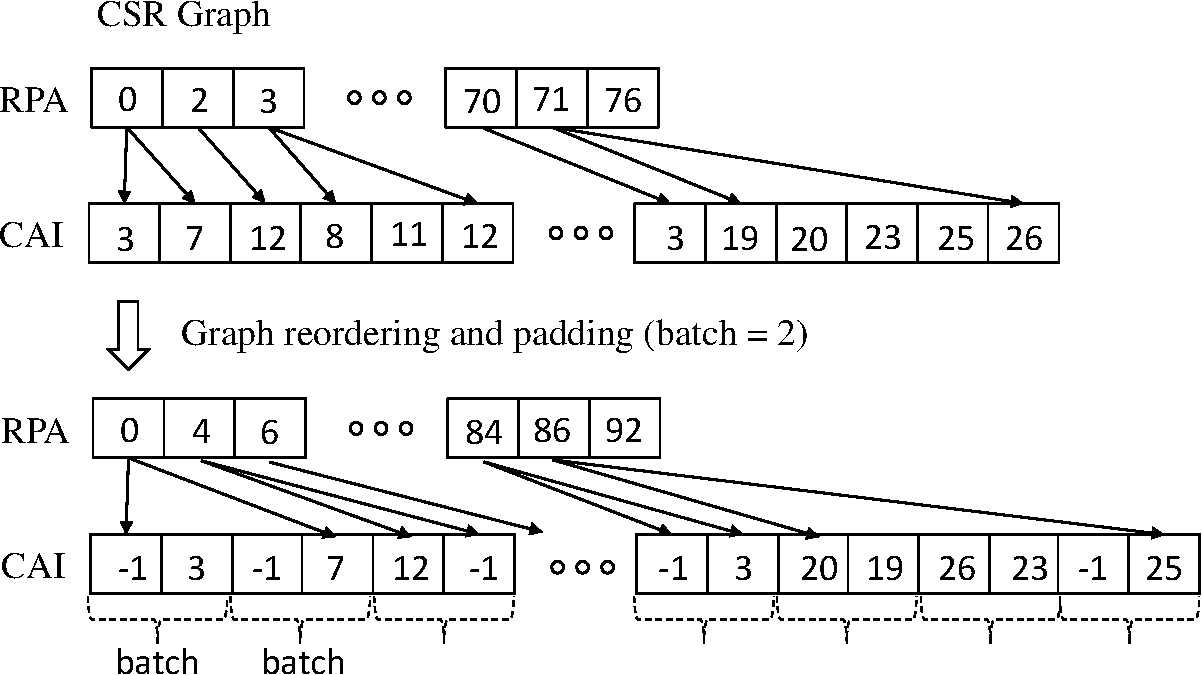
\includegraphics[width=0.75\linewidth]{graph-reorder}}
    \caption{CSR layout after the graph reordering and padding}
\label{fig:graph-reorder}
\end{figure}

\subsection{Bitmap partition and parallel access}
\subsection{CPU assisted data reorganization}
\subsection{Batch write}

\subsection{Optimized BFS structure}
Optimized BFS structure is presented in Figure \ref{fig:opt-bfs}.
\begin{figure}
	\center{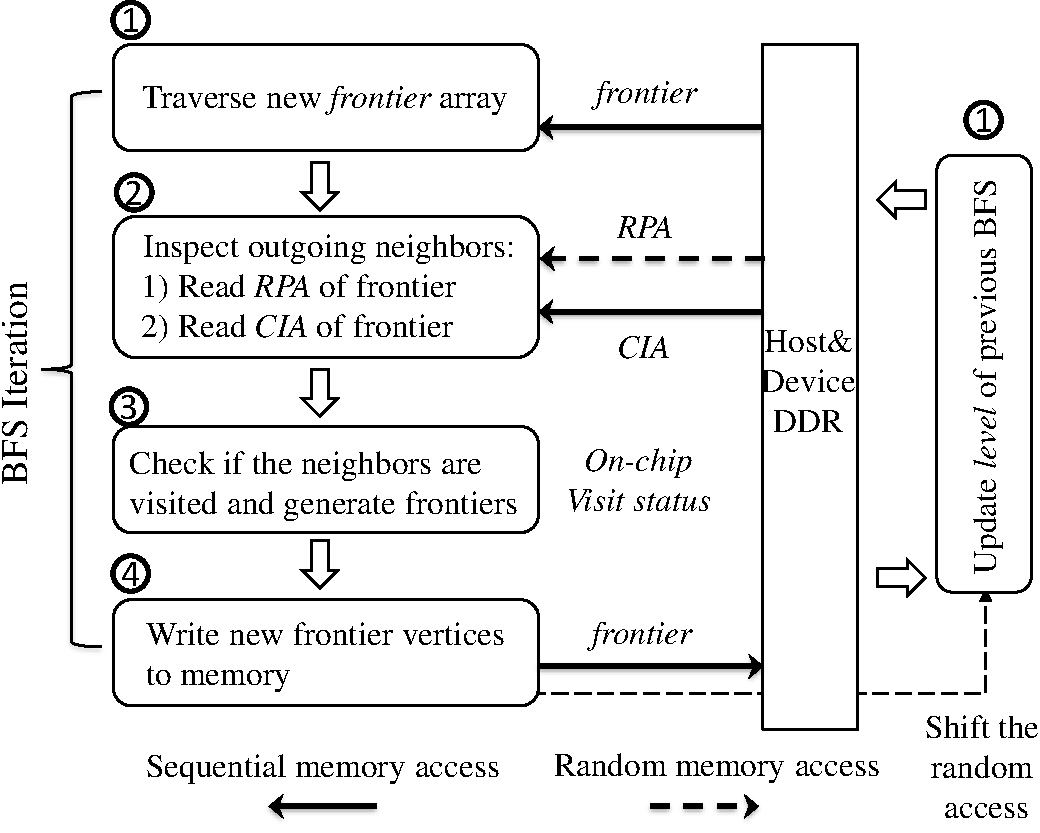
\includegraphics[width=0.85\linewidth]{opt-bfs}}
    \caption{Optimized BFS pipeline}
\label{fig:opt-bfs}
\end{figure}

\subsection{Theoretical performance analysis}
In this sub section, we analyzed the theoretical performance.
